\documentclass[11pt,a4paper]{article}
\usepackage[utf8]{inputenc}
\usepackage[english]{babel}

\usepackage{graphicx}
\usepackage[english]{babel}
\usepackage[margin=0.85in]{geometry}
\usepackage{amsmath}
\usepackage{natbib}
\usepackage{hyperref}
\bibliographystyle{plainnat}
\usepackage{setspace}


% These are the configurable settings
% Please change them to make it fit your course
\def \institute {Institute / project name}
\def \authors { Youri Hoogstrate, \institute }

\def \servers {
\begin{itemize}
	\item \url{https://usegalaxy.org/}
	\item \url{https://bioinf-galaxian.erasmusmc.nl/galaxy/}
\end{itemize}
}
\def \datalibrarydirintroduction {
	TraIT Galaxy Training Materials
		$\rightarrow$
	TraIT Galaxy Training - 1: Introduction to Galaxy
}

\def \datalibrarydirrnaseqtuxedo {
	TraIT Galaxy Training Materials
		$\rightarrow$
	TraIT Galaxy Training - 3: RNASeq Tuxedo Pipeline
}

\def \datalibrarydirrnaseqadvanced {
	TraIT Galaxy Training Materials
		$\rightarrow$
	TraIT Galaxy Training - 5: Advanced RNA-Seq Analysis
}
% Configurations should be changed in this file

\begin{document}
\title{ \textit{\institute}\text{ }Galaxy Training: Introduction to Galaxy \\
{ \large This practical aims to familiarize a user with the Galaxy user interface. It will teach how to perform basic tasks such as uploading data, running tools, working with histories, creating workflows, and sharing data. } }

\author{ \authors }
\maketitle

%\newpage
%\tableofcontents
%\newpage

%\doublespacing

\section*{Introduction}
This manual is inspired by the Galaxy-101 pages available at \url{https://github.com/nekrut/galaxy/wiki/Galaxy101-1} and \url{https://usegalaxy.org/u/galaxyproject/p/galaxy-variant-101}.
Due to the rapid development of Galaxy screenshots and results may be out of date. If you experience something like this, please report it as a bug at \url{https://github.com/ErasmusMC-Bioinformatics/galaxy-courses/issues}.


% It should describe:
% - server address(es)
% - whether to use specific training accounts or register one
% - a notice until when the server will be available or whether it will be accessible after the course
% - funding related notices
\section*{Preparations}
\subsection*{Open Galaxy}
Please open a web browser and navigate to your assigned Galaxy server:

\servers

\subsection*{Register for an account}
In the top menu bar, go to User and then choose Register (fig. \ref{fig:registration}). After registration, click on Analyze data in the top menu to return to the main screen.

\begin{figure}
 \center
  
\includegraphics[scale=0.6]{../figures/register_icon_1}
  \caption{\small{ The icons used in Galaxy to go to the registration page }}
  \label{fig:registration}
\end{figure}% Preparations should describe how to access which server

\subsection*{Getting started}
The time is there to play with Galaxy. The main screen consists of three parts, on the left is the list of available tools, on the right side the history pane showing the analysis you have performed so far and in the middle panel the tools and data visualizations (fig. \ref{fig:organization_layout}).

\begin{figure}
 \center
  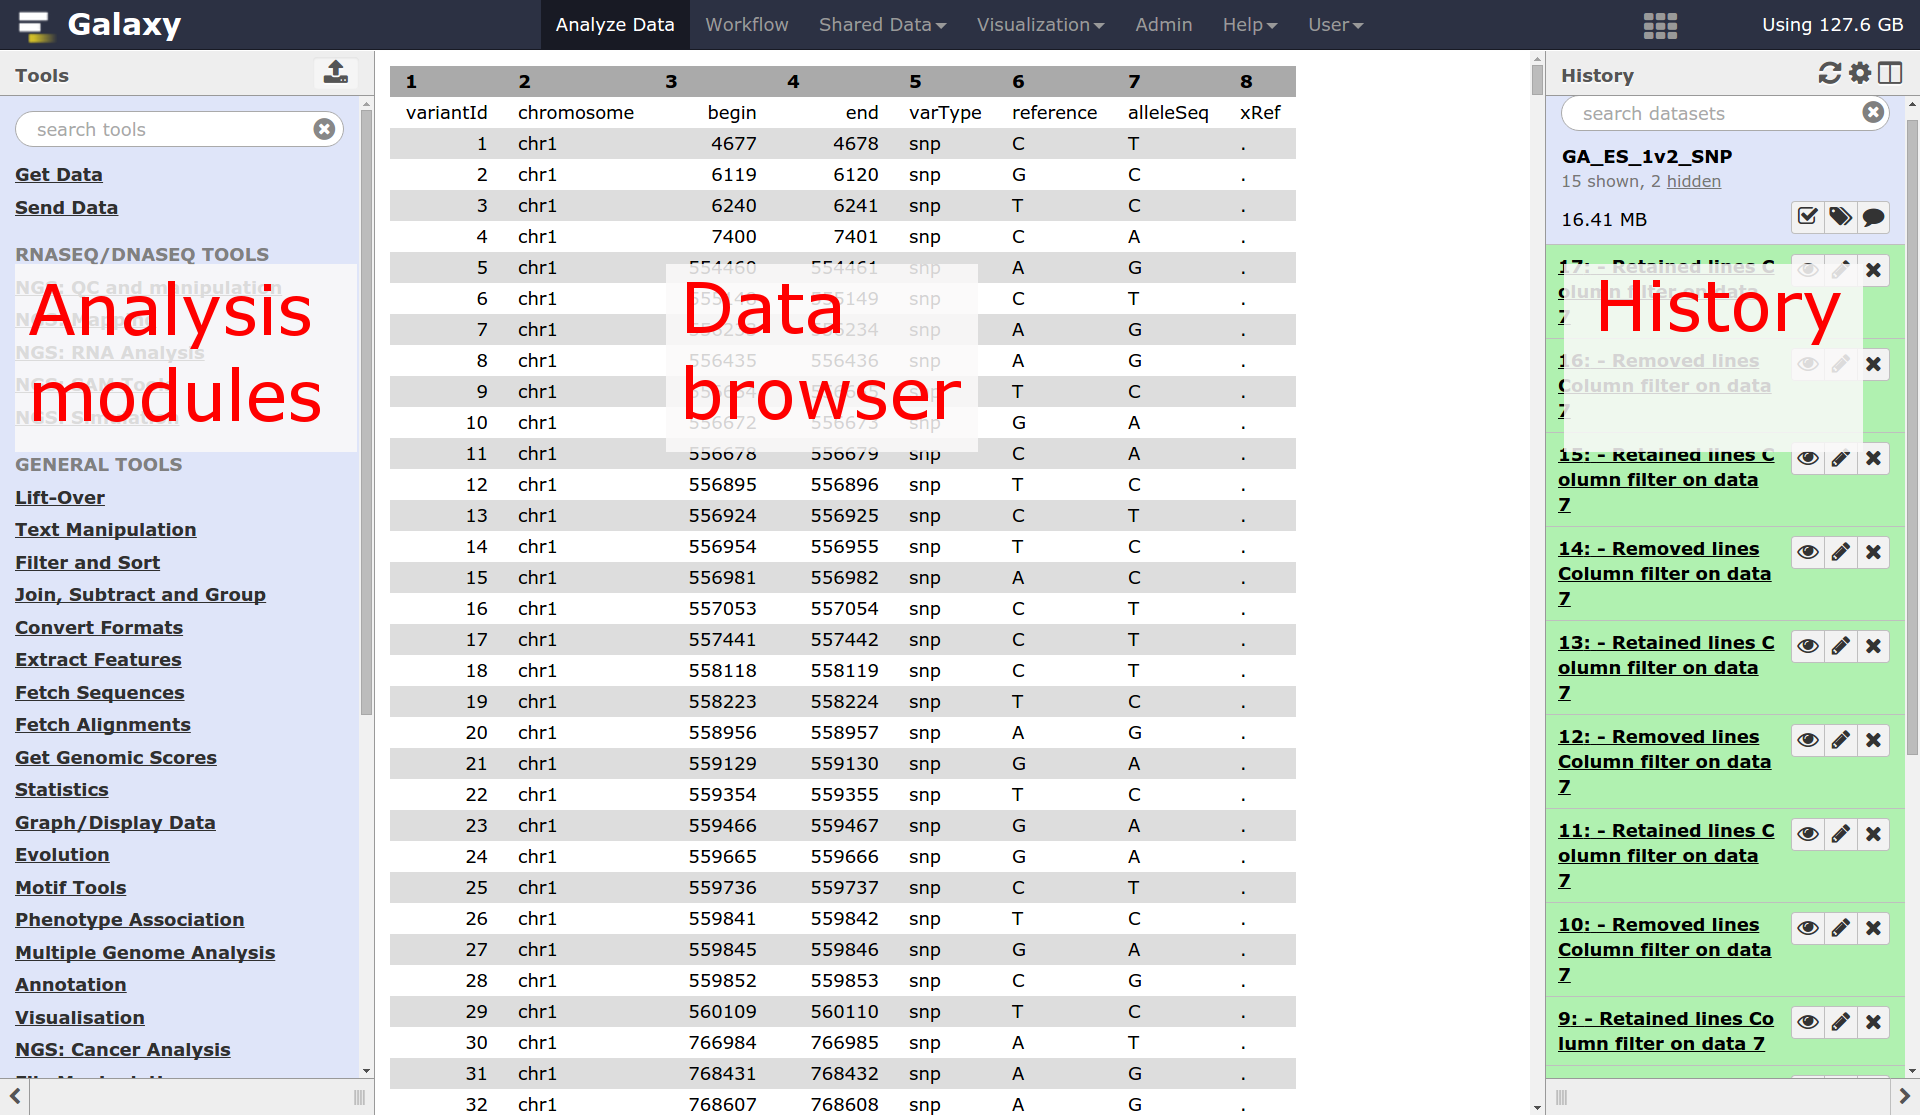
\includegraphics[width=\textwidth]{figures/galaxy_layout}
  \caption{\small{ The organization of Galaxy: on the left side the analysis modules like tools and workflows, in the middle page the data or the controls of the analysis modules, and on the right side the history items. }}
  \label{fig:organization_layout}
\end{figure}

\section*{Galaxy 101: The first thing you should try}
In this very simple example we will introduce you to bare basics of Galaxy:
\begin{itemize}
	\item Getting data from UCSC
	\item Performing simple data manipulation
	\item Understanding Galaxy's Tool and History system
	\item Creating and editing workflows
	\item Applying workflows to your data
\end{itemize}
Suppose you get the following question: ``\textit{Mom (or Dad) ... Which coding exon has the highest number of single nucleotide polymorphisms on chromosome 22?}''. You think to yourself ``\textit{Wow! This is a simple question ... I know exactly where the data is (at UCSC) but how do I actually compute this?}'' The truth is, there is really no
straightforward way of answering this question in a time frame comparable to the attention span of a 7-year-old. Well ... actually there is and it is called Galaxy. So let's try it...

\section{Getting data from UCSC genome browser}
First thing we will do is to obtain data from UCSC by clicking ``Get Data $\rightarrow$ UCSC Main'':\\
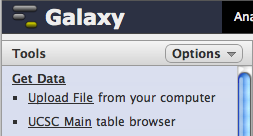
\includegraphics[scale=0.65]{figures/101_01} \\
You will see UCSC (in older versions of Galaxy it is embedded in the middle pane) which looks like this:\\
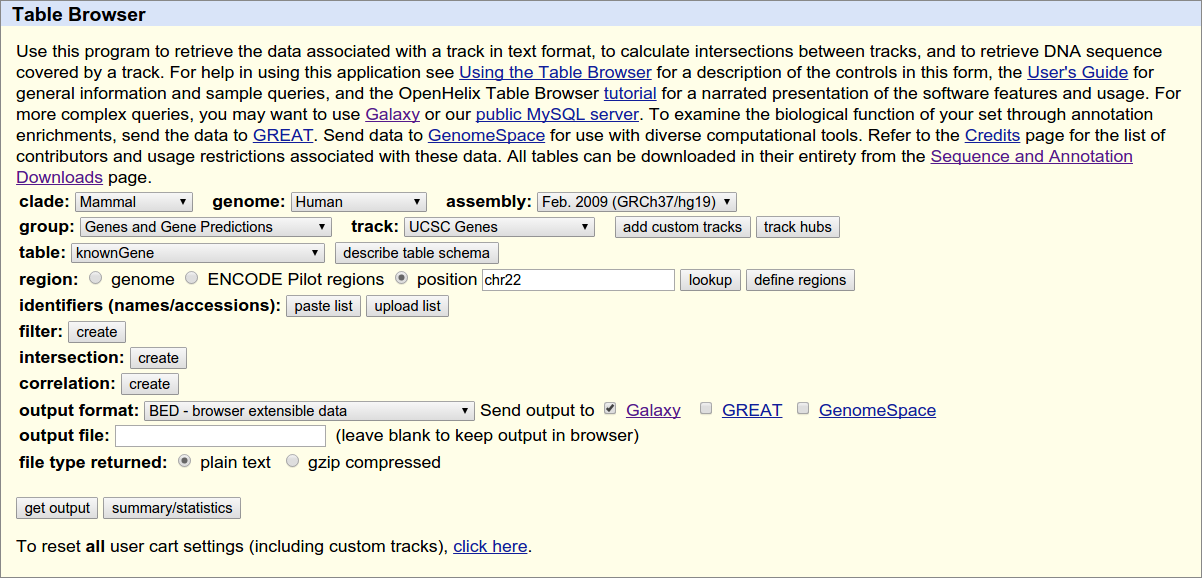
\includegraphics[width=\textwidth]{figures/101_02} \\
Make sure that your settings are exactly the same as shown on the screen (in particular, \textbf{assembly} should be set to \textit{Feb. 2009 (GRCh37/hg19}, \textbf{position} should be set to ``chr22'', \textbf{output format} should be set to ``BED - browser extensible data'', and ``Galaxy'' should be checked by Send output to option). Click \textit{get output} and you will see the next screen:\\
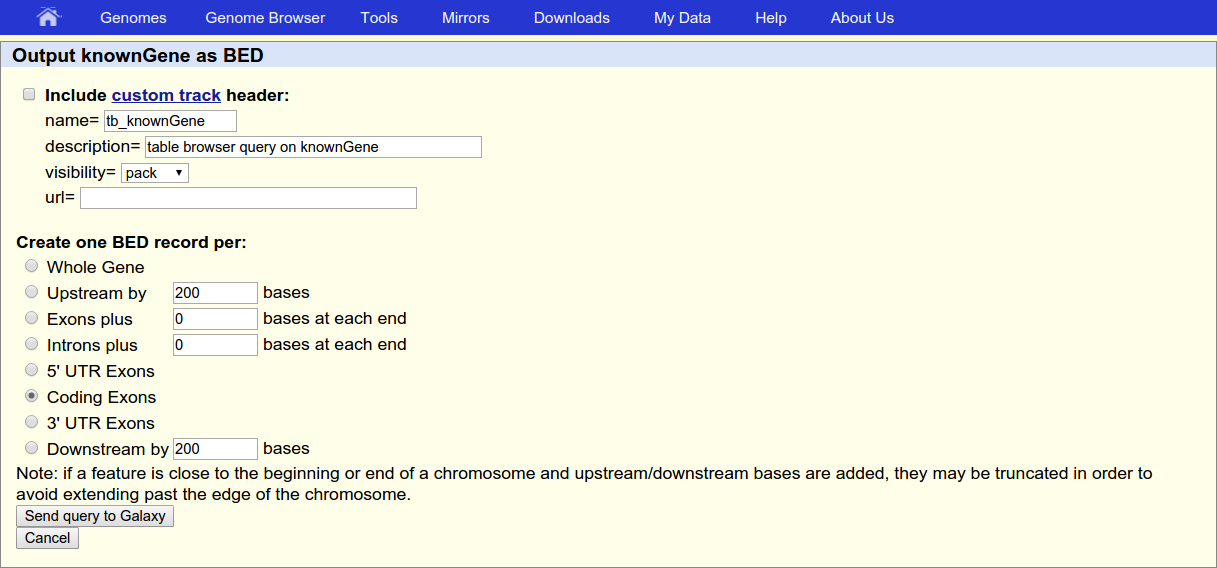
\includegraphics[width=\textwidth]{figures/101_03}\\
Make sure \textbf{Create one BED record per} is set to ``Coding Exons'' and click \textbf{Send Query to Galaxy}. After this you will see your first History Item in Galaxy's right pane. It will go through gray (preparing) and yellow (running) states to become green:\\
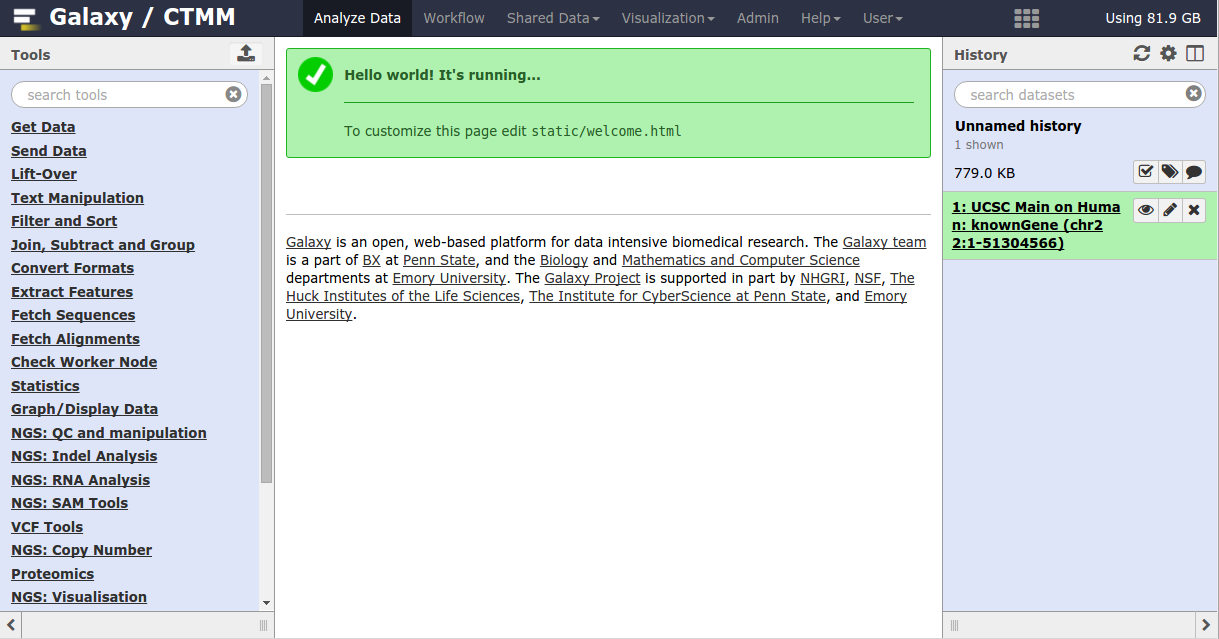
\includegraphics[width=\textwidth]{figures/101_04}\\
To view the contents of the file, click on the eye icon.

\subsection{Gettings SNPs}
Now is the time to obtain SNP data. This is done almost exactly the same way. First thing we will do is to again click on ``Get Data $\rightarrow$ UCSC Main'':\\
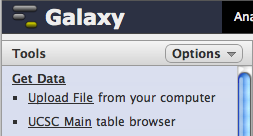
\includegraphics[scale=0.65]{figures/101_01}\\
But now change group to ``Variation'' to obtain the SNPs. It may be that newer versions of \textbf{Common SNPs ($\ldots$)} are available. It is not a big deal to select another one (if the one in the figure below is not available anymore), but the results will be slightly different. After selection the page will look like this:\\
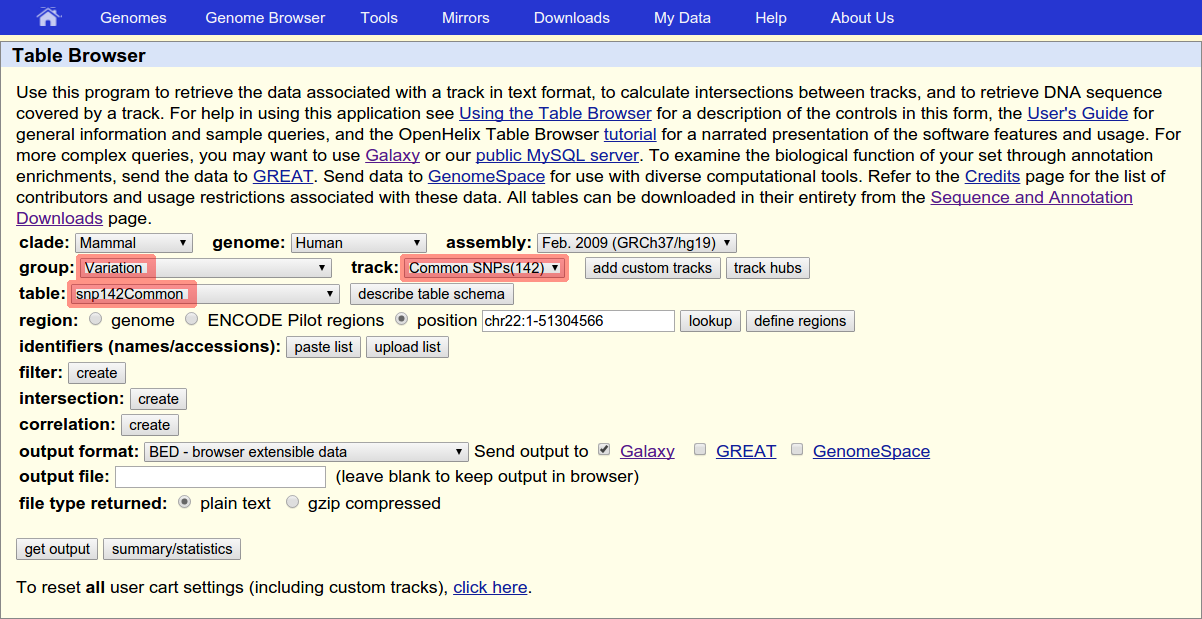
\includegraphics[width=\textwidth]{figures/101_06}\\
Then click \textbf{get output} to find a menu similar to this:\\
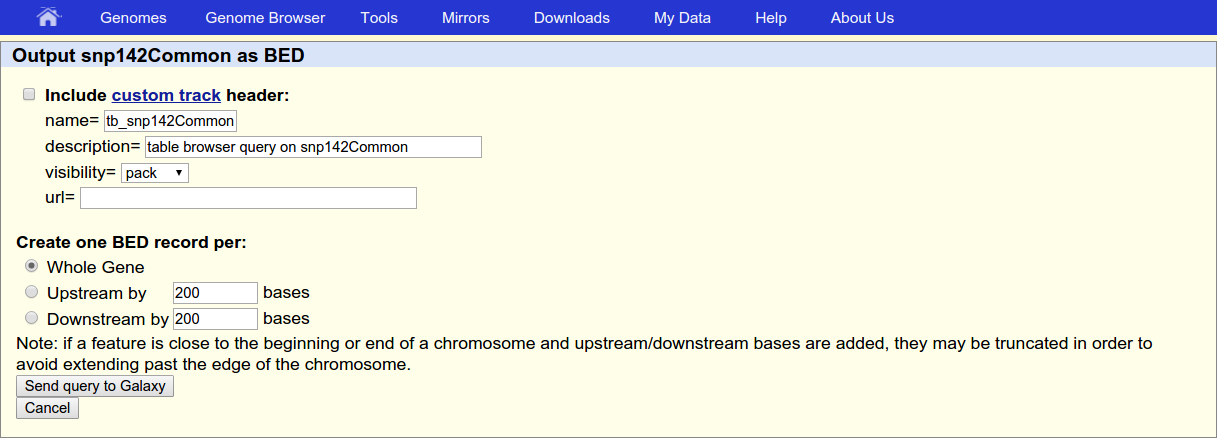
\includegraphics[width=\textwidth]{figures/101_07}\\
You need to make sure that \textbf{Whole Gene} is selected (``Whole Gene'' here really means ``Whole Feature'') and click \textbf{Send Query to Galaxy}. You will get your second item in the history:\\
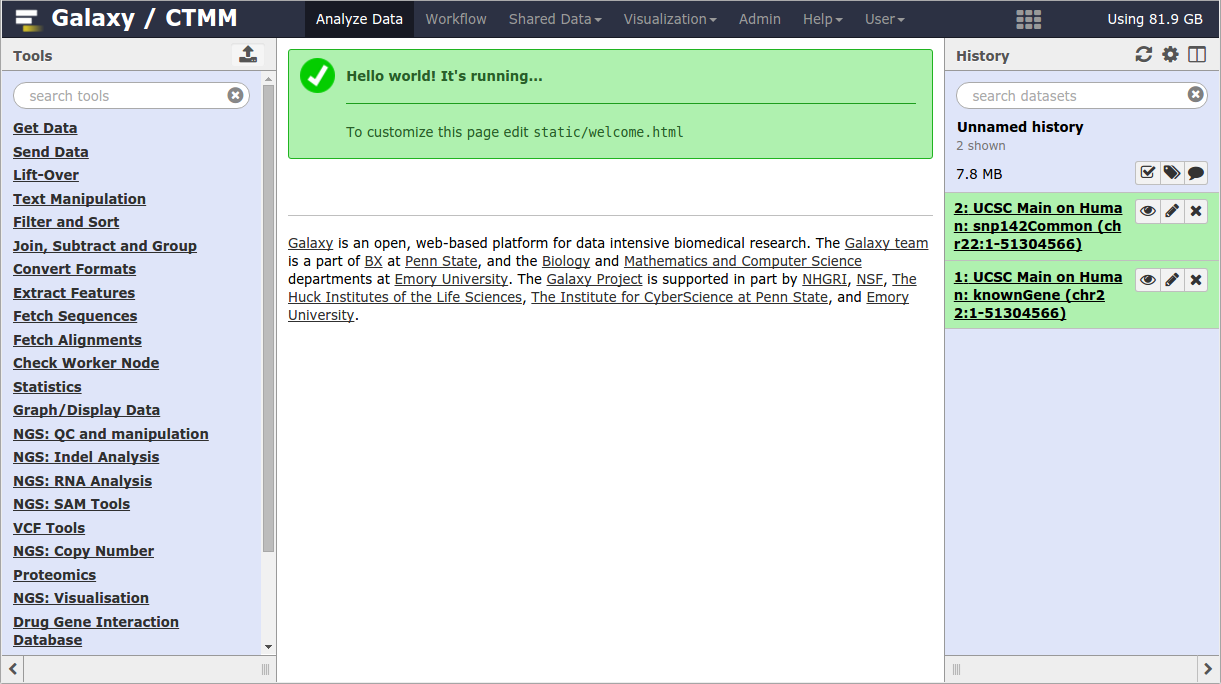
\includegraphics[width=\textwidth]{figures/101_08}\\
Now we will rename the two history items to ``Exons" and ``SNPs" by clicking on the Pencil icon adjacent to each item. Also we will rename history to "Galaxy 101" (or whatever you want) by clicking on "Unnamed history" so everything looks like this:\\
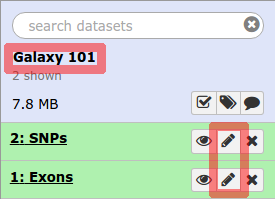
\includegraphics[scale=0.65]{figures/101_09}\\
\textbf{Note}: If the import from UCSC takes too long or something else went wrong, the files can still be found as shared data library in Galaxy. Browse the following directories \textit{
\datalibrarydirintroduction}
, and select the files named ``SNPs'' and ``Exons'', choose ``Import to current history'' and click ``Go''. In more recent versions of Galaxy you only have to click ``to History". Click on ``Analyze Data'' on the top menu bar to return to your analysis:\\
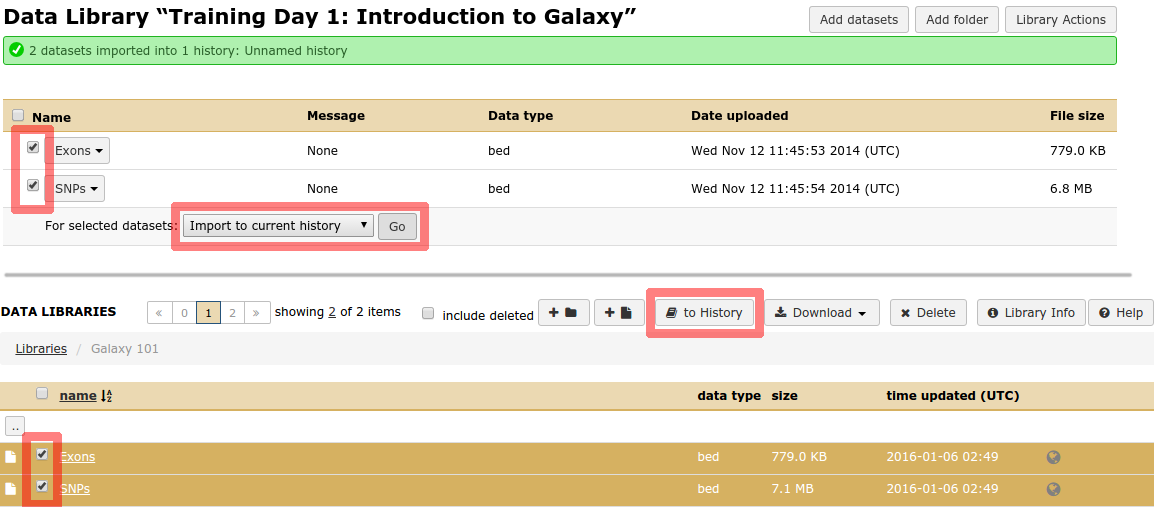
\includegraphics[width=\textwidth]{figures/101_10}\\

%\newpage

\section{Finding Exons with the highest number of SNPs}
\subsection{Joining exons with SNPs}
Let's remind ourselves that our objective was to find which exon contains the most SNPs. This first step in answering this question will be joining exons with SNPs (a fancy word for printing exons and SNPs that overlap side by side). This is done using the tool ``\underline{Join} the intervals of two datasets side-by-side''.
Different servers will have this tool available under different sections. This accounts for all tools actually. Therefore it is recommended to search for a tool in the search bar in the left top. Once you have found it you can join the SNPs into the exons by selecting the following:\\
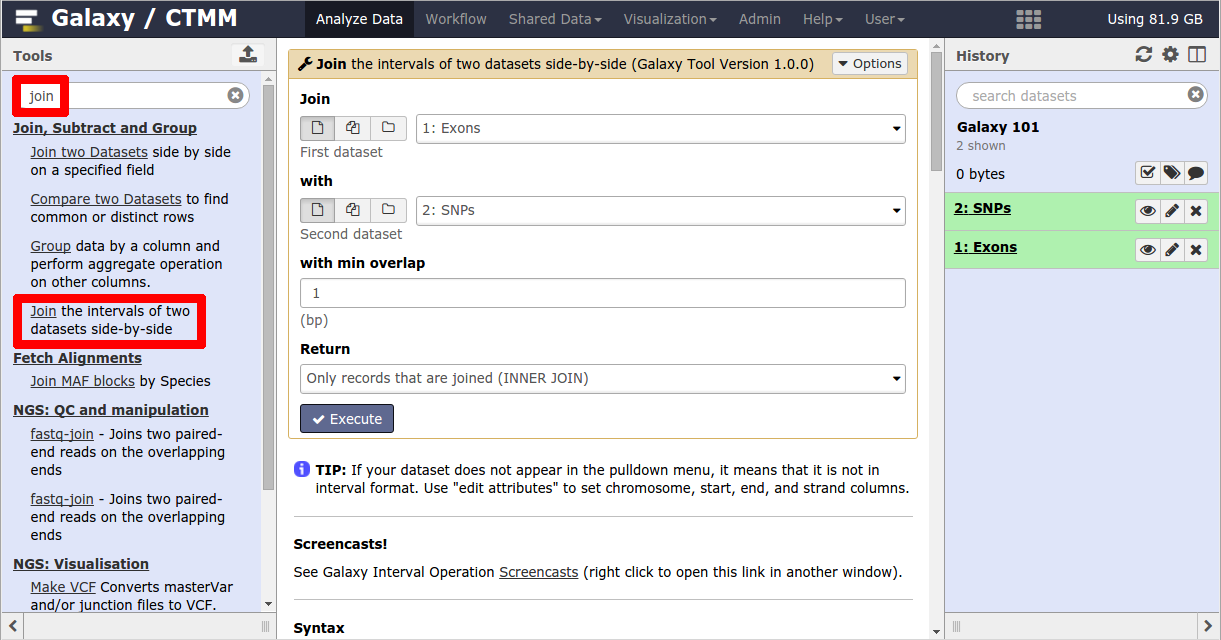
\includegraphics[width=\textwidth]{figures/101_11}\\
\textbf{Note}: if you scroll down on this page, you will find an explanation about the tool. Make sure your exons are first and SNPs are second and click \textbf{Execute}. You will get the third history item, changing color over time. When it is \textbf{gray}, it \textbf{is scheduled} for analysis. When it is \textbf{yellow}, it \textbf{is performing} the analysis and when it \textbf{is green}, the analysis \textbf{has completed}. \\
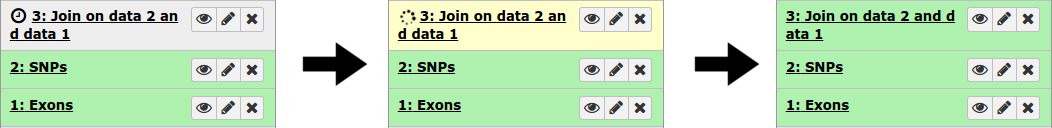
\includegraphics[width=\textwidth]{figures/101_12}\\
\textbf{General notice: when jobs are not finished (yellow or gray) ADDING MORE JOBS DOES NOT MAKE ANALYSIS GO QUICKER!!!}\\
\\
If you did everything correctly, the first lines of the data will be:
{\scriptsize
\begin{verbatim}
chr22	16277747	16277885	uc002zlh.1_cds_6_0_chr22_16277748_r	0	-	chr22	16277851	16277852	rs200742649	0	+
chr22	16277747	16277885	uc010gqp.2_cds_6_0_chr22_16277748_r	0	-	chr22	16277851	16277852	rs200742649	0	+
chr22	16287253	16287885	uc010gqp.2_cds_10_0_chr22_16287254_r	0	-	chr22	16287338	16287339	rs199952431	0	+
chr22	16287253	16287885	uc010gqp.2_cds_10_0_chr22_16287254_r	0	-	chr22	16287850	16287851	rs72485235	0	+
chr22	16287253	16287885	uc010gqp.2_cds_10_0_chr22_16287254_r	0	-	chr22	16287648	16287649	rs201243560	0	+
\end{verbatim}}
$ \\ $
Let's take a look at this dataset. The first six columns correspond to exons. The last six correspond to SNPs. You can see that exon with ID \verb|uc002zlj.1_cds_8_0_chr22_16287254_r| contains three SNPs with IDs \verb|rs199952431|, \verb|rs200073113| and \verb|rs201840700|.
\subsection{Counting the number of SNPs per exon}
We've just seen that exon \verb|uc002zlj.1_cds_8_0_chr22_16287254_r| is repeated three times in the above dataset. Thus we can easily compute the number of SNPs per exon by simply counting the number of repetitions of name for each exon. This can be easily done with the ``Group'' tool:\\
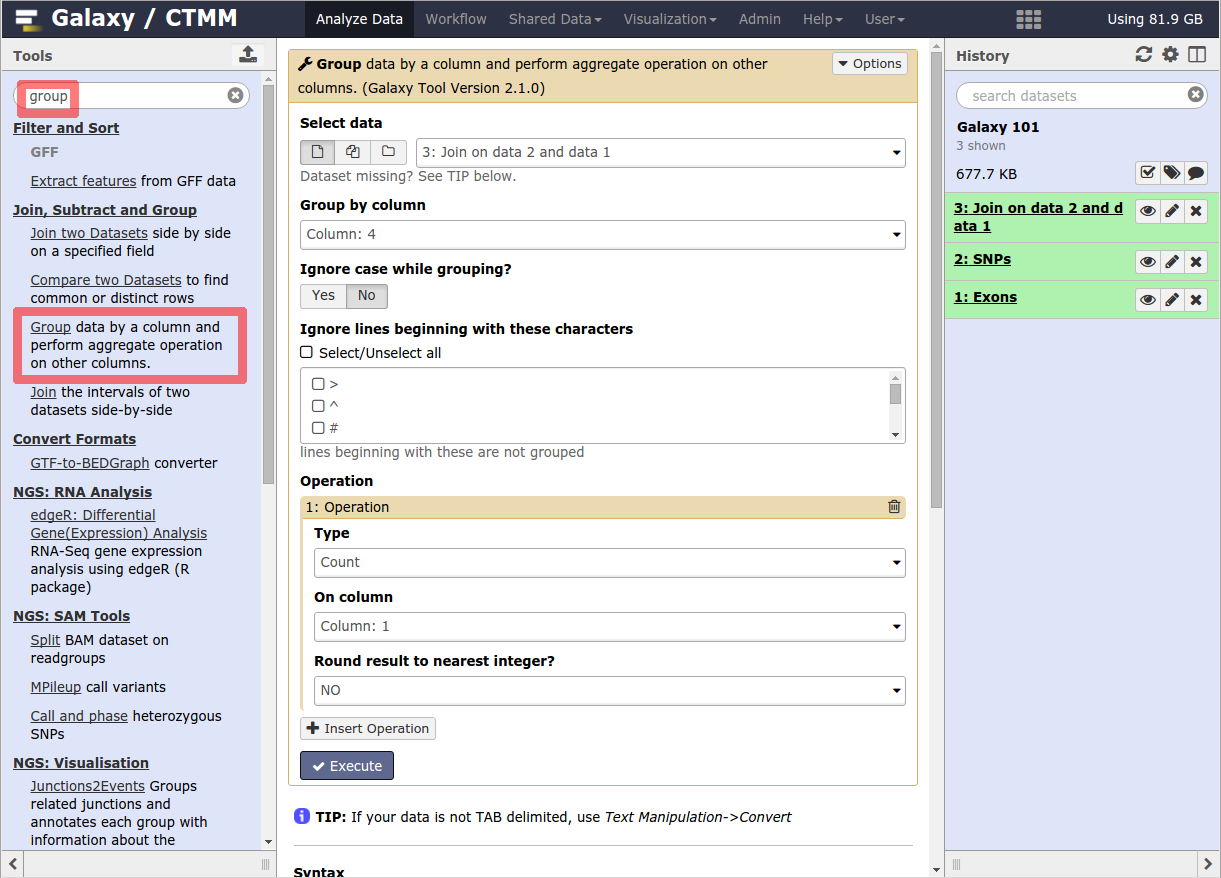
\includegraphics[width=\textwidth]{figures/101_13}\\
Click \textbf{Execute} to do the grouping. Your history will look something like this:\\
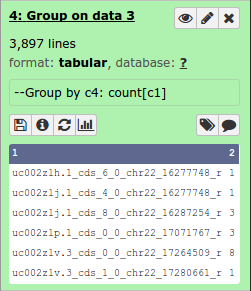
\includegraphics[scale=0.65]{figures/101_14}\\
If you look at the above image you will see that the result of grouping (dataset \#4) contains two columns. The first column contains the exon names while the second contains the number of times this name has been repeated in dataset \#3 (i.e. number of SNPs within that exon).
\subsection{Sorting exons by SNP count}
To see which exon has the highest number of SNPs we can simply sort dataset \#4 on the second column in descending order. This can be done with the ``Sort'' tool:\\
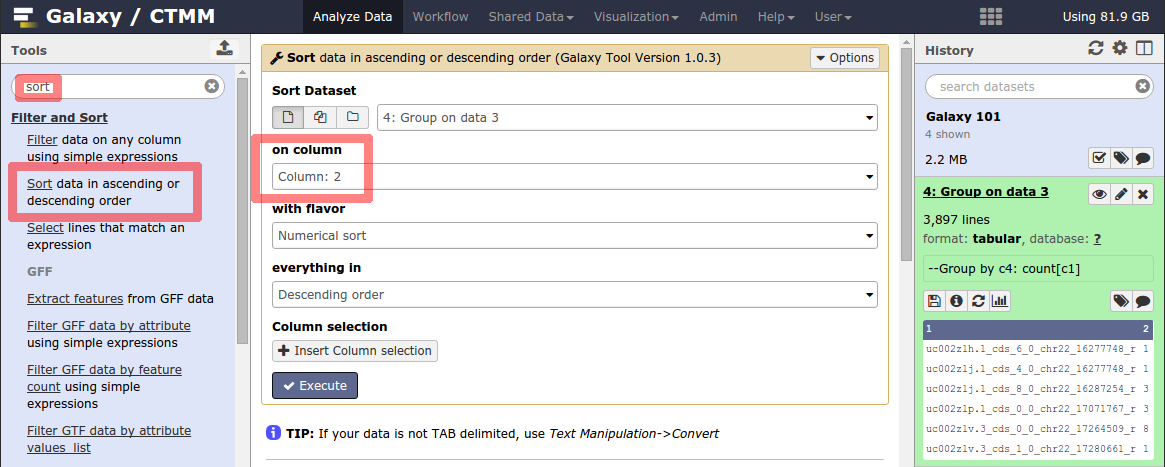
\includegraphics[width=\textwidth]{figures/101_15}\\
This will generate the a history item in which you can now see that the highest number of SNPs per exon is ...:\\
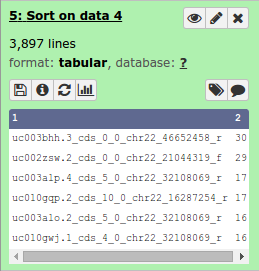
\includegraphics[scale=0.65]{figures/101_16}\\
\subsection{Selecting top five}
To select the top five exons with the highest number of SNPs we will use the tool ``\underline{Select first} lines from a dataset''. Set the number to 5 and press \textbf{Execute} to produce a history item that will contain these five lines:\\
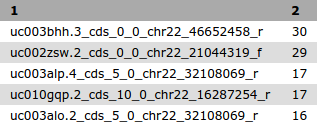
\includegraphics[width=\textwidth]{figures/101_17}\\
\subsection{ Recovering exon info and displaying data in genome
browsers}
Now we know that in this dataset the five top exons contain between 16 and 30 SNPs, but what else can we learn about them? To know more we need to get back the positional information (genomic coordinates) of these exons.
This information was lost at the grouping step and now all we have is just two columns. To get the genomic coordinates back we will match the names of exons in dataset \#6 (column 1) against names of the exons in the original dataset \#1 (column 4). This can be done with ``\underline{Compare two Datasets} to find common or distinct rows'' tool using the following settings:\\
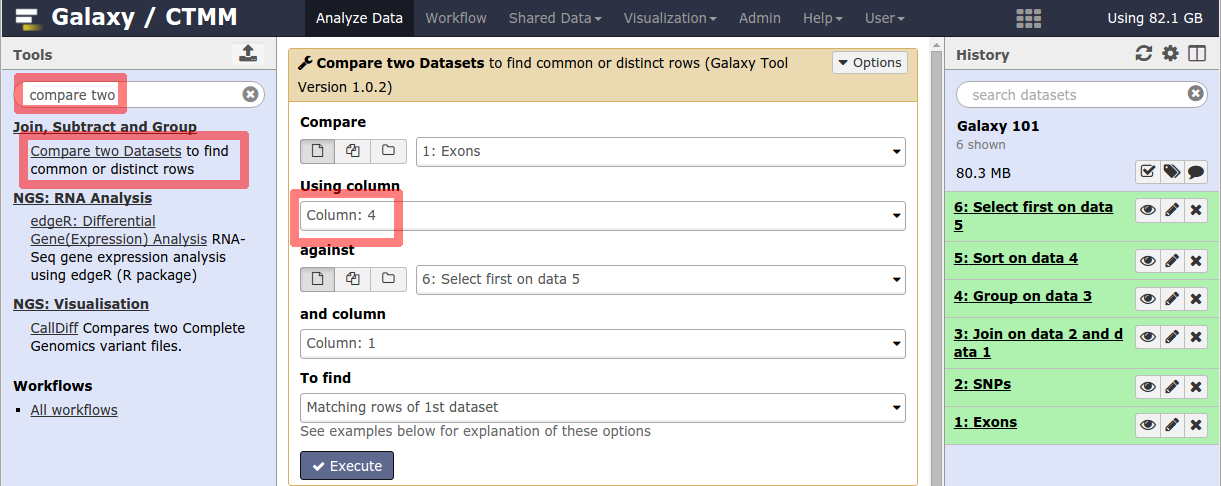
\includegraphics[width=\textwidth]{figures/101_18}\\
This will add a new dataset to the history:\\
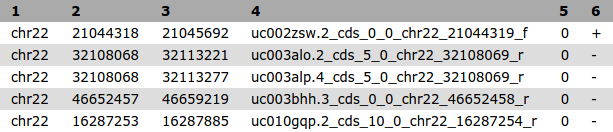
\includegraphics[scale=0.65]{figures/101_19}\\
A good way to learn about these exons is to look at their genomic surrounding. This can be done by using genome browsers. 
Therefore, first, we have to tell galaxy to which reference genome this data belongs (hg19) as follows:\\
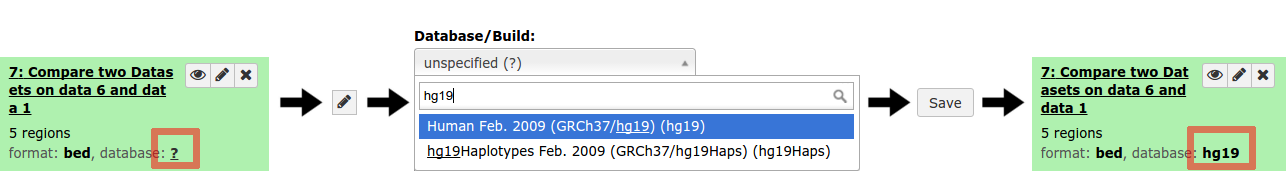
\includegraphics[width=\textwidth]{figures/101_20}\\
To visualize the data in UCSC, click on ``display at UCSC main'' at the history item if you are at a public galaxy instance.
When you are at at protected galaxy instance, download the file and upload it at UCSC as custom track (My Data $\rightarrow$ Custom Tracks). This will upload the data to UCSC as custom track (to
see your regions look at ``User Supplied Track'' (track near the top)). In UCSC enter coordinates: \verb|chr22:32,102,914-32,118,375| to get a view that centres around the second top-5 exon like this:\\
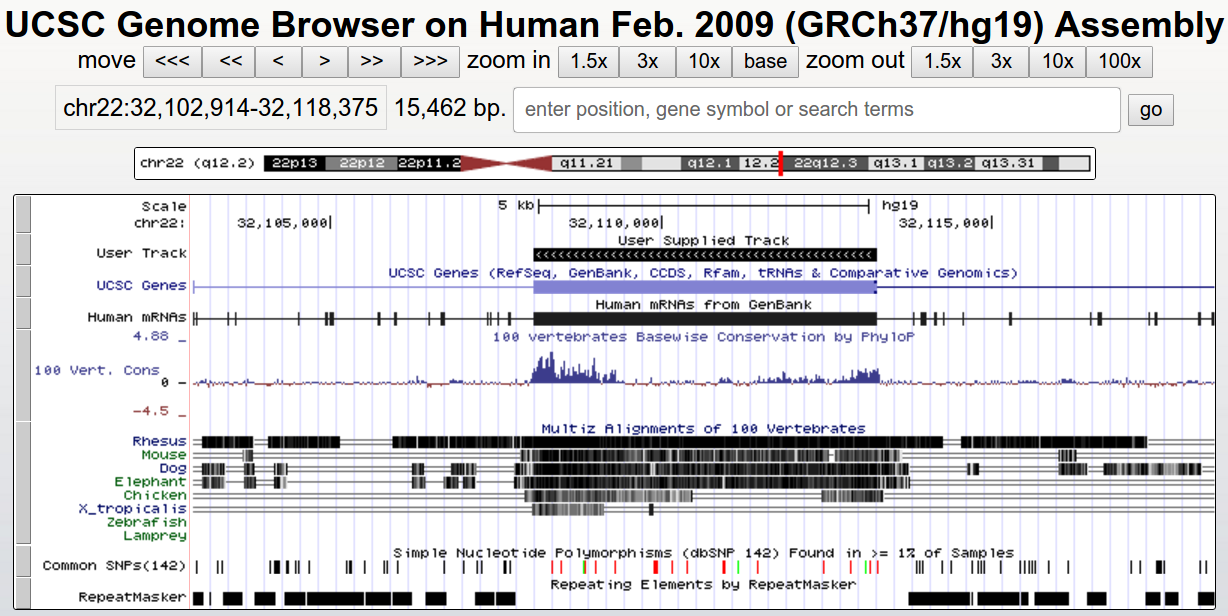
\includegraphics[width=\textwidth]{figures/101_21}\\
\section{Understanding histories}
In Galaxy your analyses live in histories such as your current one. Histories can be very large, you can have as many histories as you want, and all history behaviour is controlled by the \textbf{Options} button on the top of the History pane (gear symbol):\\
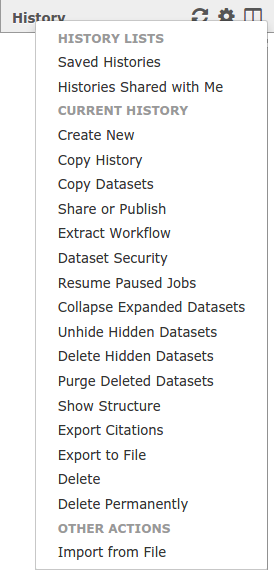
\includegraphics[scale=0.65]{figures/101_22}\\
If you create a new history, your current history does not disappear. If you would like to list all of your histories just choose Saved Histories and you will see a list of all your histories in the center pane:\\
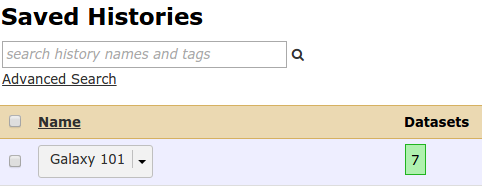
\includegraphics[scale=0.65]{figures/101_23}\\
\section{Converting histories into workflows}
\subsection{Extracting workflow}
When you look carefully to your history, you can see that it contains \textbf{all} steps of our analysis, from the beginning to the end.
By building this history we have actually built a complete record of our analysis with Galaxy preserving all parameter settings applied at every step. Wouldn't it be nice to just convert this history into a workflow that we'll be able to execute again and again? This can be done by clicking on Options (gear) button and selecting Extract Workflow option:\\
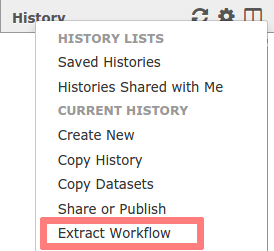
\includegraphics[scale=0.65]{figures/101_24}\\
The center pane will change as shown below and you will be able to choose which steps to include/exclude and how to name the newly created workflow. In the example it was named \textit{Find exons with highest number of SNPs}:\\
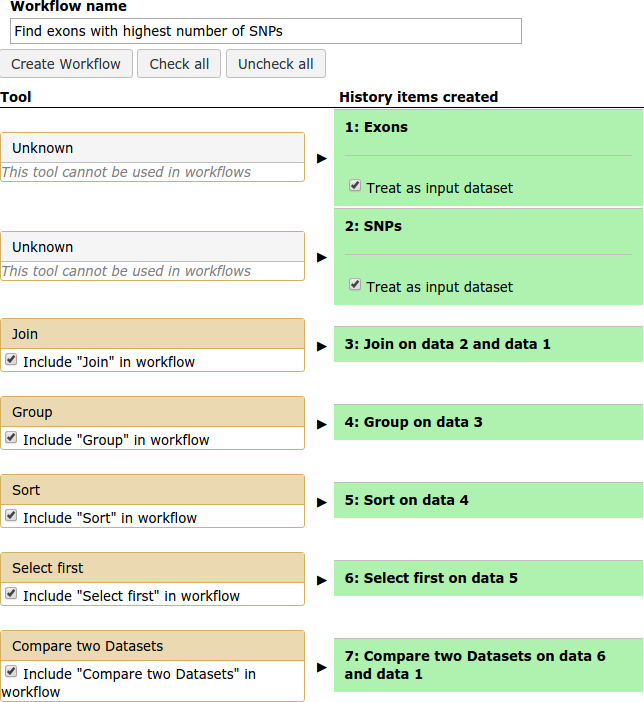
\includegraphics[scale=0.55]{figures/101_25}\\
Once you click \textbf{Create Workflow} you will get the following message: \textit{Workflow ``Find exons with highest number of SNPs''}. But where did it go? Click on \textbf{Workflow} at the top of Galaxy interface and you will a list of all workflows with ``Find exons with highest number of SNPs'' listed at the top:\\
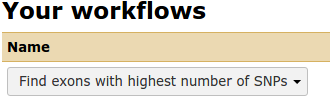
\includegraphics[scale=0.55]{figures/101_26}\\
\subsection{Opening workflow editor}
If you click on a triangle adjacent to the workflow's name you will see the following dialogue:\\
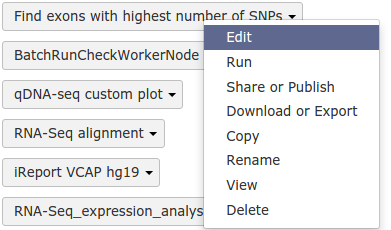
\includegraphics[scale=0.55]{figures/101_27}\\
Click \textbf{Edit} and the workflow editor will launch. It will allow you to examine and change settings of this workflow as shown below. Note that the box corresponding to the ``\textit{Select First}'' tool is selected (highlighted with the blue border) and you can see parameters of this tool on the right pane. This is how you can view and change parameters of all tools involved in the workflow:\\
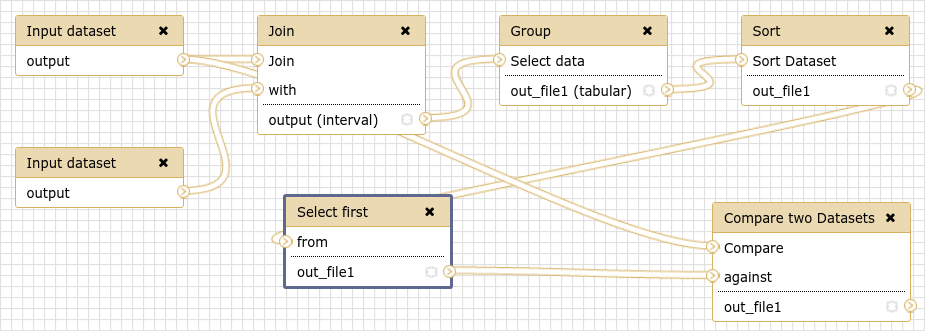
\includegraphics[width=\textwidth]{figures/101_28}\\
\subsection{Hiding intermediate steps}
When a workflow is executed, the user is usually primarily interested in the final product and not in all intermediate steps. Output files can be hidden by mousing over the small asterisk in the lower right corner of every tool box:\\
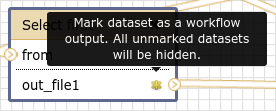
\includegraphics[scale=0.55]{figures/101_29}\\
Yet there is a catch. In a newly created workflow all steps are hidden by default and default behavior of Galaxy is that if all steps of a given workflow are hidden, then nothing gets hidden in the history. This may be
counter-intuitive, but this is done to decrease the amount of clicking if you do want to hide some steps. So if we want to hide all intermediate output files with the exception of the last one, we will click that asterisk
in last step of the workflow:\\
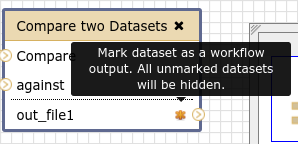
\includegraphics[scale=0.55]{figures/101_30}\\
Once you do this the representation of the workflow in the bottom right corner of the editor will change with the last step becoming orange. This means that this is the only step which will generate an output file visible in the history:\\
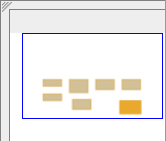
\includegraphics[scale=0.55]{figures/101_31}\\
\subsection{Renaming inputs}
Right now both inputs to the workflow look exactly the same, named ``Input dataset''. It will be very confusing which input should be exons and which should be SNPs:\\
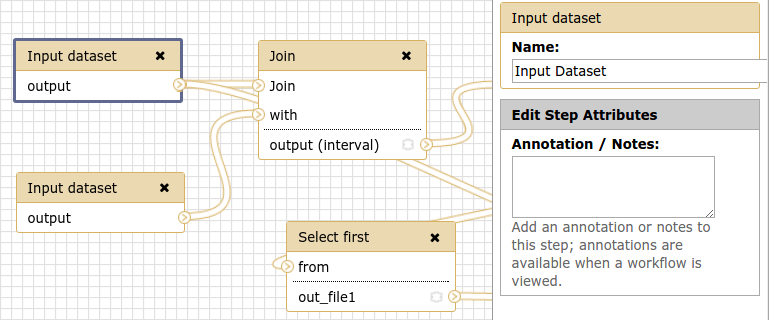
\includegraphics[scale=0.55]{figures/101_32}\\
On the image above you will see that the top input dataset (the one with the blue border) connects to the \textit{Join} tool first, so it must correspond to the exon data. If you click on this box (in the image above it is
already clicked on because it is outlined with the blue border) you will be able to rename the dataset in the right pane:\\
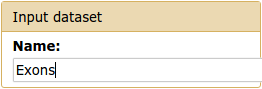
\includegraphics[scale=0.55]{figures/101_33}\\
Then click on the second input dataset and rename it to ``Features''. This would make the workflow a bit more generic, which will be useful later in this tutorial.
\subsection{Renaming inputs}
Finally let's rename the workflow's output. For this click on the last dataset (``Compare two Queries''). Scroll down in the right pane, expand the ``Add Actions'' dialog and select ``Rename Dataset'':\\
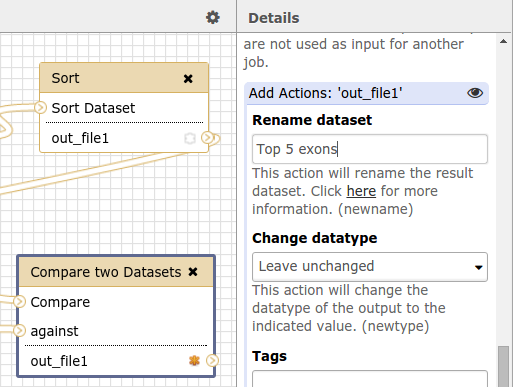
\includegraphics[scale=0.55]{figures/101_34}\\
\subsection{Save! It is important...}
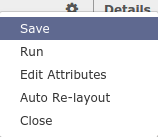
\includegraphics[scale=0.55]{figures/101_35}
\section{Run workflow on different data}
Now that we have a workflow, let's use it on some different data. For example, let's find exons with the highest number of repetitive elements.
\subsection{Create a new history}
Before we start let's create a new history by clicking \textbf{Options} and selecting \textbf{Create New}. Let's get the chr22 exons from the data library again, as well as a list of repetitive elements (which were
also obtained from UCSC table browser):\\
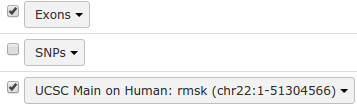
\includegraphics[scale=0.55]{figures/101_36}
\subsection{Start the Workflow}
At this point you will have two items in your history: one with exons and one with repeats. First, click on the \textit{Workflow} link at the top of Galaxy interface, mouse over ``Find exons with highest number of SNPs'' (or whatever you named your workflow), click on the arrow and press \textbf{run}:
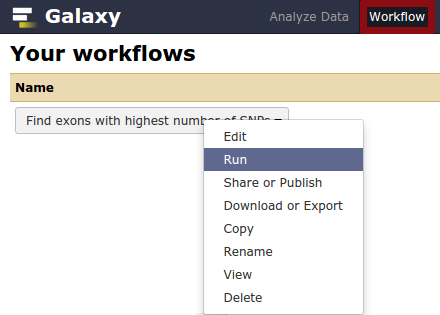
\includegraphics[scale=0.55]{figures/101_37}\\
The center pane will change to allow you launching the workflow. Select appropriate datasets for Exons and Repeats inputs as shown below, scroll down, and click Run workflow:\\
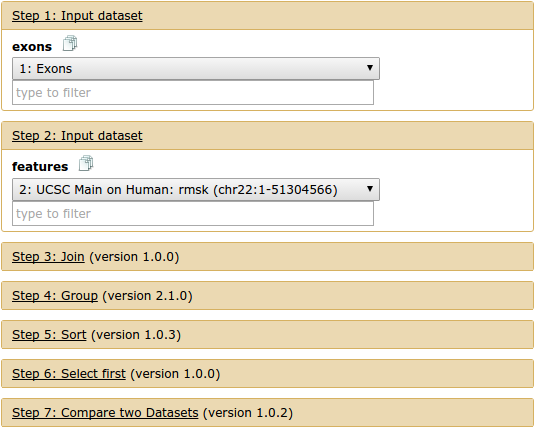
\includegraphics[scale=0.55]{figures/101_38}\\
Once the workflow has started you will initially be able to see all its steps (you may need to click the refresh button at the top of your history if the steps do not show up):\\
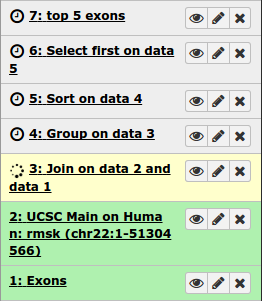
\includegraphics[scale=0.55]{figures/101_39}\\
Note that because all intermediate steps of the workflow were hidden, once it is finished you will only see final dataset \#7. If we want to view the intermediate files, we can view the hidden datasets by selecting ``\textbf{Include Hidden datasets}'' from the history options menu.
\subsection{Share your work}
I believe the most important part of galaxy comes at the end of an analysis. When you have published striking findings it is important that other researchers are able to reproduce your in silico experiment. Galaxy allows to share, or publish, your created workflows, histories with other galaxy users, with other users or with the entire outside world. Thus, this allows you to share your software and data together. To share a history, click on the gear symbol in the history pane and select \textbf{Share or Publish}. On this page you can do 3 things:
\begin{enumerate}
	\item \textbf{Make accessible via Link.} This generates a link that you can give out to others. Anybody with this link will be able to view your history (even without a Galaxy account).
	\item \textbf{Publish History.} This will not only create a link, but will also publish your history. (i.e. Your history will now appear
 under Shared Data $\rightarrow$ Published Histories)
	\item \textbf{Share with Individual Users.} This will share the history only with specific users on the Galaxy instance. Enter their email address (which they used to register their account in Galaxy)
\end{enumerate}

Challenge:
\begin{itemize}
	\item Share one of your histories with your neighbour, or publish it.
	\item See if you can do the same with your workflow!
\end{itemize}

%\bibliographystyle{natbib}
%\bibliographystyle{plainnat}

%\newpage

\vspace{-1.5em}
\bibliography{references}

\end{document}